\subsection{Reading curves from images}

I have found that more often than not we are required to measure $T_u$ and $T_g$
by  hand from visual plots, without access to the underlying data.  To  overcome
the need to  print  out  the plots onto paper and -- inaccurately -- measure the
data by hand, an algorithm for extracting this data from an image was developed.

\begin{figure}
    \centering
    \begin{subfigure}{.3\textwidth}
        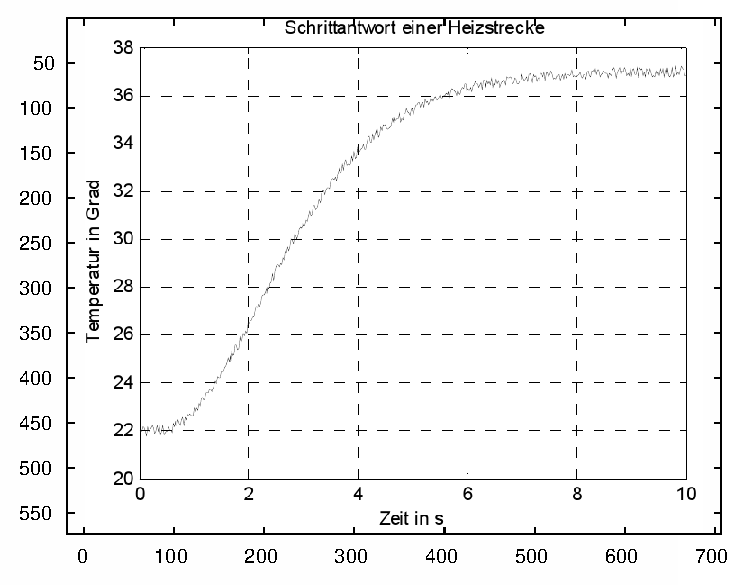
\includegraphics[width=.95\linewidth]{images/plant}
        \caption{Typical image of a plant}
        \label{fig:image:plant}
    \end{subfigure}
    \begin{subfigure}{.3\textwidth}
        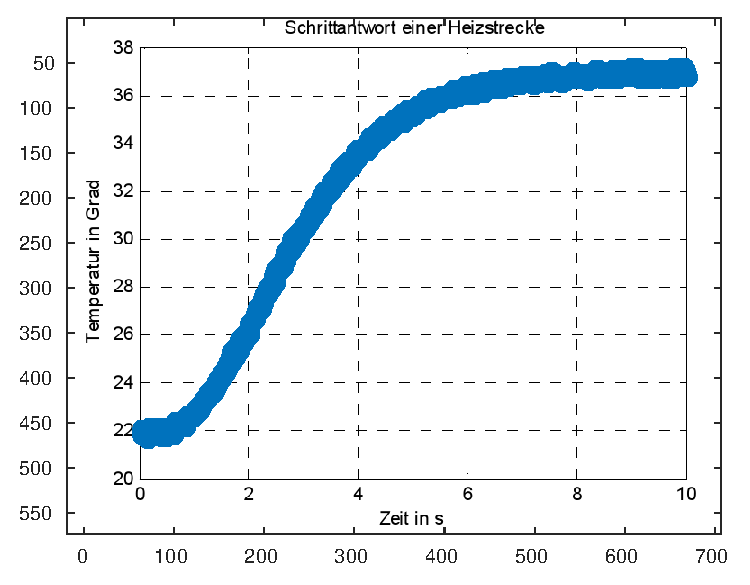
\includegraphics[width=.95\linewidth]{images/scatter_raw}
        \caption{XY scatter of detected data}
        \label{fig:image:scatter_raw}
    \end{subfigure}
    \begin{subfigure}{.3\textwidth}
        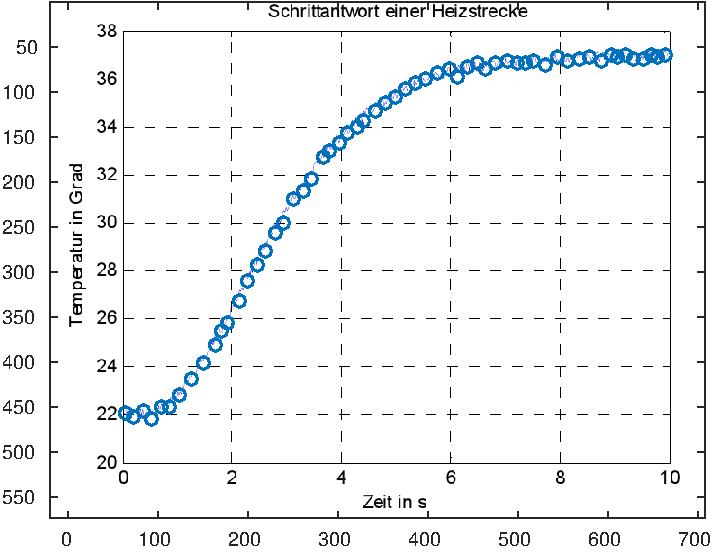
\includegraphics[width=.95\linewidth]{images/scatter_decimated_50}
        \caption{Decimated by 50}
        \label{fig:image:scatter_dec}
    \end{subfigure}
    \caption{Process of importing curve data from an image}
\end{figure}

The algorithm is quite simple: The image data is imported into HSV colour space.
In  the majority of cases, the grid and background will be white, black or  some
grey-scale. The data on the other hand will have a specific colour, which allows
us to first detect  what  the  colour is and then filter the image by hue to get
all data points that have a similar colour.

If the plot happens to be black and white with no colour, then it is possible to
filter  the  data  using  the   ``value''   component   from   the   HSV   data.

The resulting data is usually noisy, but statistically evenly distributed, which
makes  decimation  very easy: Just select every nth data point.  The  data  from
\ref{fig:image:scatter_raw} was decimated by a factor of 50, resulting in figure
\ref{fig:image:scatter_dec}.

